\subsection{Mobile development}

\subsubsection{Frameworks}

\paragraph{PhoneGap}
PhoneGap takes applications written with web technologies and wraps them in
a different ``web view'' application for each of the mobile platforms you
target. In essence, it's like saving a web page on your phone and opening
it in a browser without window chrome. This allows you to ``write once, run
everywhere''. Additionally, the PhoneGap framework wraps the native APIs of
different platforms in a single JavaScript API which is made available to
developers using PhoneGap. This makes PhoneGap apps potentially much more
powerful than simple web pages.

\paragraph{Backbone.js}
The JavaScript programming language does not strictly enforce any specific
architecture or code organization. Furthermore, JavaScript was initially
created so that simple interaction could be added to web pages when the web was
still an immature platform. These two factors led to a long history of poorly
structured JavaScript, or ``spaghetti code''.

Backbone.js attempts to solve this problem by introducing the MVP
(model--view--presenter) software pattern to client-side applications,
separating domain data and logic (Backbone models) from the user interface
(HTML) and mediating between the two through a presenter (Backbone view).

Backbone.js is widely used in industry and has only one dependency, the
Underscore.js library which shares the same creator as Backbone.js.
Therefore it meets our customer's requirement that we use well known
technologies that can be easily maintained.

\paragraph{Jasmine}
Jasmine is a unit testing framework for JavaScript. It advocates BDD
(behavior-driven development) in that its syntax is descriptive of what the
tested code is supposed to do and reads like a user story. Like Backbone.js,
Jasmine is widely used in industry. It is also included by default when you
create a new PhoneGap project, so presumably the two fit nicely together.

\subsubsection{Conclusions}


\begin{figure}[!ht]
\centering

\subfigure{
  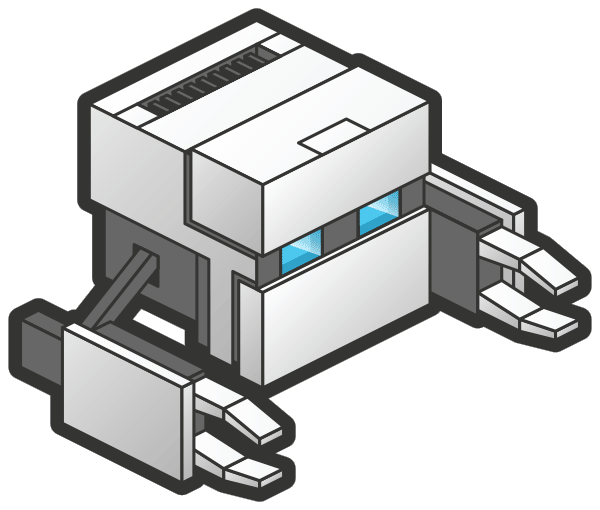
\includegraphics[scale=0.15]{pictures/phonegap}
}
\subfigure{
  
\includegraphics[scale=0.15]{pictures/backbone}
}
\subfigure{
  
\includegraphics[scale=0.9]{pictures/jasmine}
}
\caption{Phonegap, Backbone and Jasmine}
\end{figure}
